% CVPR 2022 Paper Template
% based on the CVPR template provided by Ming-Ming Cheng (https://github.com/MCG-NKU/CVPR_Template)
% modified and extended by Stefan Roth (stefan.roth@NOSPAMtu-darmstadt.de)

\documentclass[10pt,twocolumn,letterpaper]{article}

%%%%%%%%% PAPER TYPE  - PLEASE UPDATE FOR FINAL VERSION
%\usepackage[review]{cvpr}      % To produce the REVIEW version
%\usepackage{cvpr}              % To produce the CAMERA-READY version
\usepackage[pagenumbers]{cvpr} % To force page numbers, e.g. for an arXiv version

% Include other packages here, before hyperref.
\usepackage{graphicx}
\usepackage{amsmath}
\usepackage{amssymb}
\usepackage{pifont}
\usepackage{booktabs}
\usepackage{multirow}
\usepackage{url}


% It is strongly recommended to use hyperref, especially for the review version.
% hyperref with option pagebackref eases the reviewers' job.
% Please disable hyperref *only* if you encounter grave issues, e.g. with the
% file validation for the camera-ready version.
%
% If you comment hyperref and then uncomment it, you should delete
% ReviewTempalte.aux before re-running LaTeX.
% (Or just hit 'q' on the first LaTeX run, let it finish, and you
%  should be clear).
\usepackage[pagebackref,breaklinks,colorlinks]{hyperref}


% Support for easy cross-referencing
\usepackage[capitalize]{cleveref}
\crefname{section}{Sec.}{Secs.}
\Crefname{section}{Section}{Sections}
\Crefname{table}{Table}{Tables}
\crefname{table}{Tab.}{Tabs.}


%%%%%%%%% PAPER ID  - PLEASE UPDATE
\def\cvprPaperID{*****} % *** Enter the CVPR Paper ID here
\def\confName{CVPR}
\def\confYear{2022}


\begin{document}

%%%%%%%%% TITLE - PLEASE UPDATE
\title{Attack MDE}

% \author{First Author\\
% Institution1\\
% Institution1 address\\
% {\tt\small firstauthor@i1.org}
% % For a paper whose authors are all at the same institution,
% % omit the following lines up until the closing ``}''.
% % Additional authors and addresses can be added with ``\and'',
% % just like the second author.
% % To save space, use either the email address or home page, not both
% \and
% Second Author\\
% Institution2\\
% First line of institution2 address\\
% {\tt\small secondauthor@i2.org}
% }
\author{xxx
\\ School of Computer Science and Engineering, 
Sun Yat-sen University, China\\{\tt\small \{panm9\}@mail2.sysu.edu.cn}}

\maketitle

%%%%%%%%% ABSTRACT
\begin{abstract}
\end{abstract}

\section{Introduction}
Monocular Depth Estimation is a crucial 3D scene perception algorithm. 
Trapped by the lack of sufficient geometric constraints, 
MDE is still an ill-posed problem. With the rapid development of 
Deep Neural Networks(DNNs), MDE has emerged many excellent works 
in recent years. However, according to Szegedy's 
research~\cite{Szegedy_2014_ICLR}, DNNs are 
prone to be attacked by adversarial examples: when a imperceptibly 
small perturbation is added to an input image, the classifier 
based on DNNs will classify the image into a wrong category with high probability. 
This property has been verified not only on classification tasks, 
but also on logical regression tasks, such as semantic segmentation and 
object recognition. MDE also failed to get rid of this dilemma.

As a kind of 3D scene perception algorithm, MDE needs to be 
robust and reliable, so that when an attack occurs in automatic 
driving, the vehicle can still accurately perceive the depth 
of the scene. Otherwise, the damage is much more serious than 
the percentage loss in accuracy. On MDE, this problem was 
first confirmed and researched by Wong~\cite{Wong_2020_NIPS}. 
They conducted 
comprehensive and rigorous experiments to explore the impact 
of pixel attacks on MDE. Including attacking the whole 
depth map of a scene, attacking the depth map of one 
single object in the scene, and even making a specific 
object vanished completely on the depth map by 
adding perturbations. This research is pioneering and 
enlightening for attacking MDE.

\begin{figure}
	\centering
	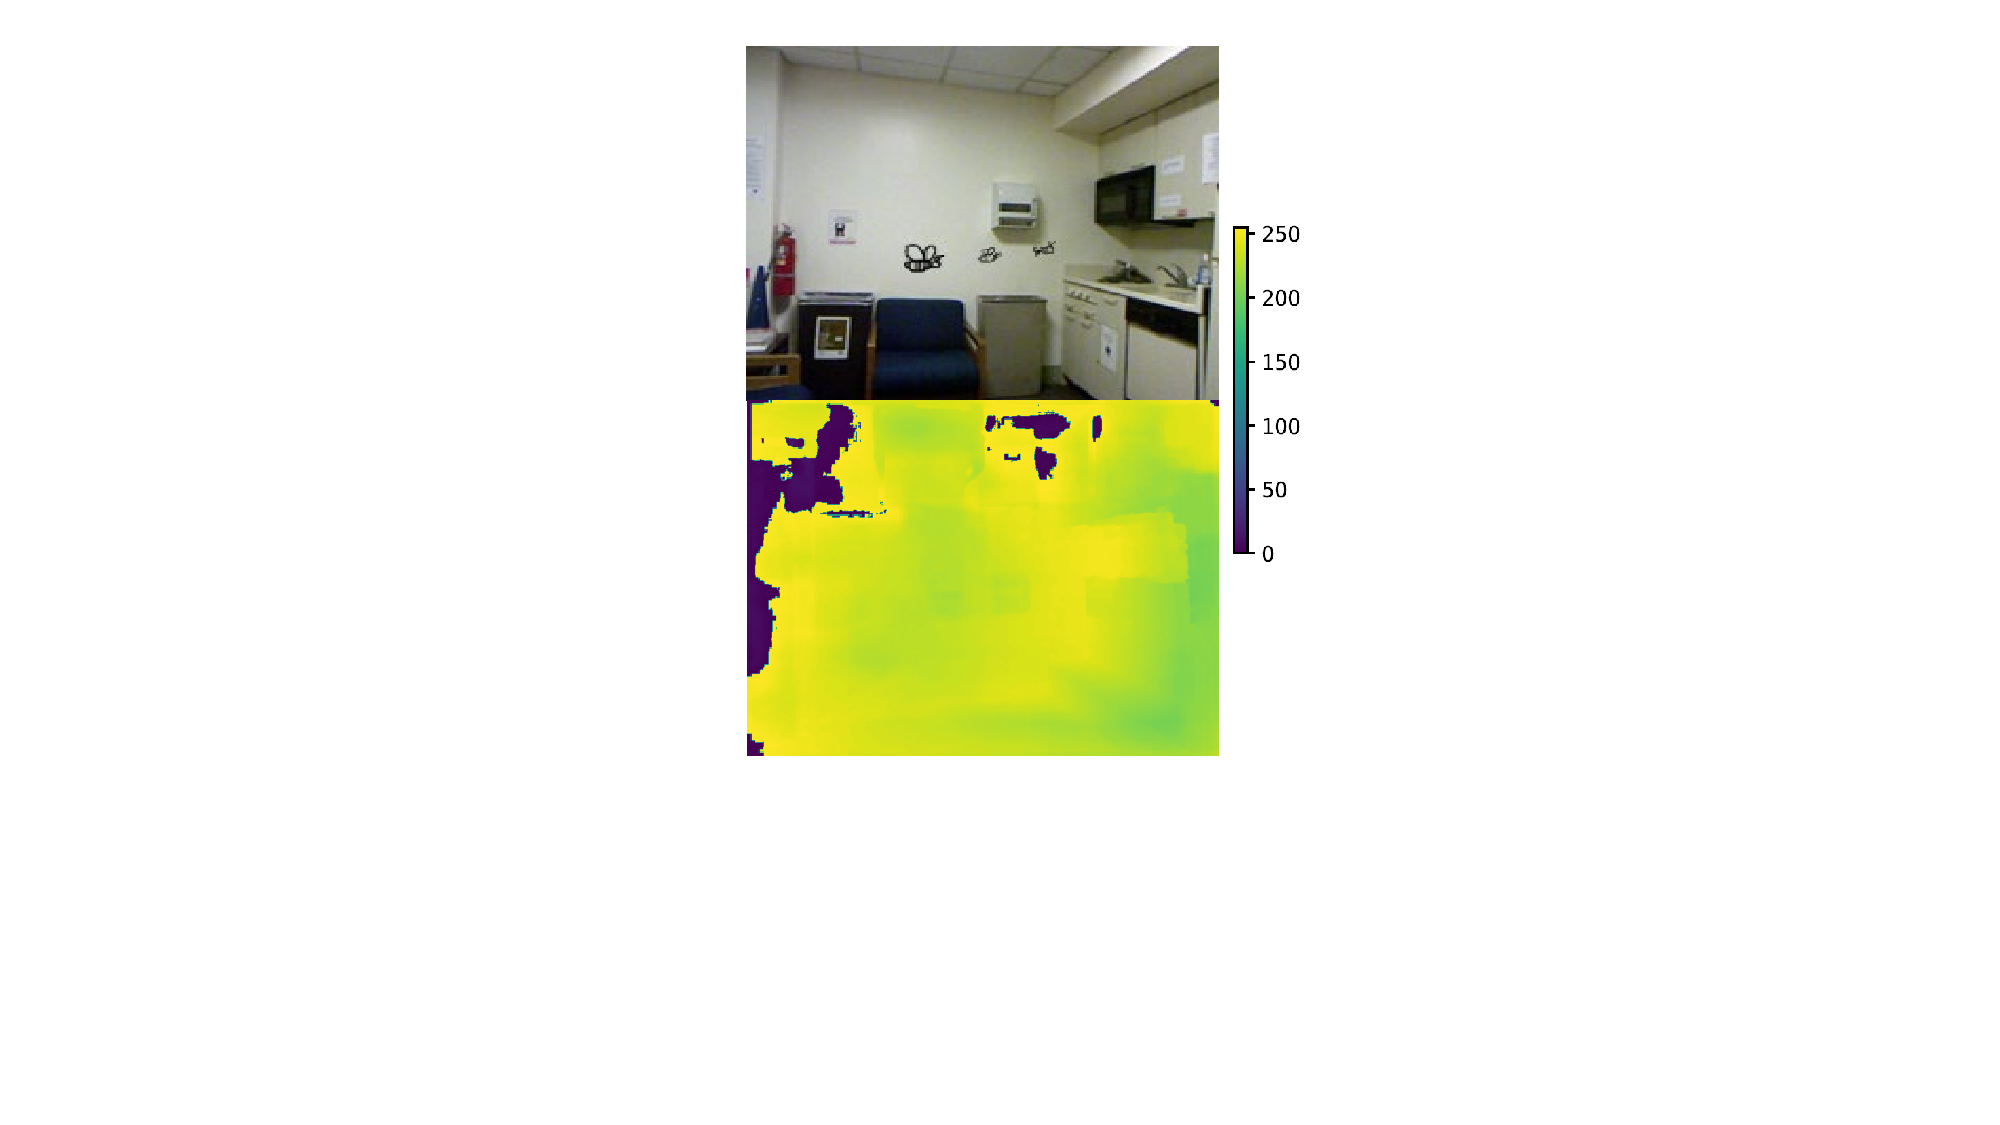
\includegraphics[width=0.45\textwidth]{imgs/effect_preview.pdf}
	\caption{we have achieved a considerable 
	attack success rate While taking into account the concealment and 
	physical implementation. }
	\label[]{effect_preview}
\end{figure}
However, the study of Wong~\cite{Wong_2020_NIPS} can hardly apply 
to physical 
world, it didn't take physical attack into account. 
The perturbations used in experiments are elaborately designed, 
which are very hard to realize in the physical world. 
While attacking a scene by patch is an appropriate solution: 
sticking a patch into the scene to be attacked is much more 
reasonable and implementable.
Some researches exploit patches to attack DNNs~\cite{Brown_2017_arxiv}, 
but most of them 
didn't pay much attention on inconspicuousness. 
Abrupt and unreal patch in scenes will reveal the attack 
intention.
Indeed, some works noticed this problem and utilize 
GAN~\cite{Hu_2021_ICCV,Kong_2020_CVPR,Liu_2019_AAAI} to make patches
more naturalistic. 
This will increase time and space complexity obviously.
In this study, we take physical realizability and 
inconspicuousness into accout, design an algorithm to attack MDE.

Specifically, we design a learnable matrix, 
which can generate reasonable patches according to depth map 
automatically. The generation processes are driven by three 
learnable coefficients and don't need any extra generation networks.

contribution.

The structure in the rest of this paper is conducted as:

\section{Related Work}
In this work, patch attacks of MDE model are concentrated on, 
so a brief review of MDE and patch attacks will be 
introduced in this section.

\subsection{Monocular Depth Estimation}
\subsubsection{Supervised}
DNNs learn through the supervision of ground truth labels 
annotated artificially. Since the mapping from a single image 
to a depth map is very complicated, this supervised learning 
manner is very suitable for MDE tasks. The initial work adopts 
this \textbf{intuitive endoder-decoder} concept. 
Eigen et al.~\cite{Eigen_2014_nips} designed two hierarchical 
neural networks to predict 
the depth map in coarse and fine respectively.
A network was proposed subsequently by them~\cite{Eigen_2015_ICCV}, 
in which three 
different tasks, depth estimation, segmentation and 
normals prediction was integrated into one model.
Lee~\cite{lee_2019_arxiv} coined novel local planar guidance layers and locate 
them at different scale decoding phases. 
As a result of this, final fine depth maps are densely 
restored from small to big.
Current MDE networks are bulky and inefficient, which can not
be equipped on embedding systems. Wofk et al.~\cite{Wofk_2019_ICRA} 
proposed Fastdepth,
a light, fast MDE network.
Some researches~\cite{Li_2018_ACCV,cao_2017_CSVT,Fu_2018_CVPR} 
address this problem by formulizing it as 
a \textbf{classification} problem. 
Discrete depth labels are prepared by separating 
continuous depth value, which are then used to supervise 
the training process.
While using \textbf{relative depth information} to predict depth 
indirectly is also a effective solution.
Lee~\cite{Lee_2019_CVPR} proposed a method to predict depth from relative depth. 
They first estimate relative depth by utilizing rank-1 property, 
then the final depth maps are reconstructed through these relative 
depth maps.


\begin{figure*}[htb]
	\centering
	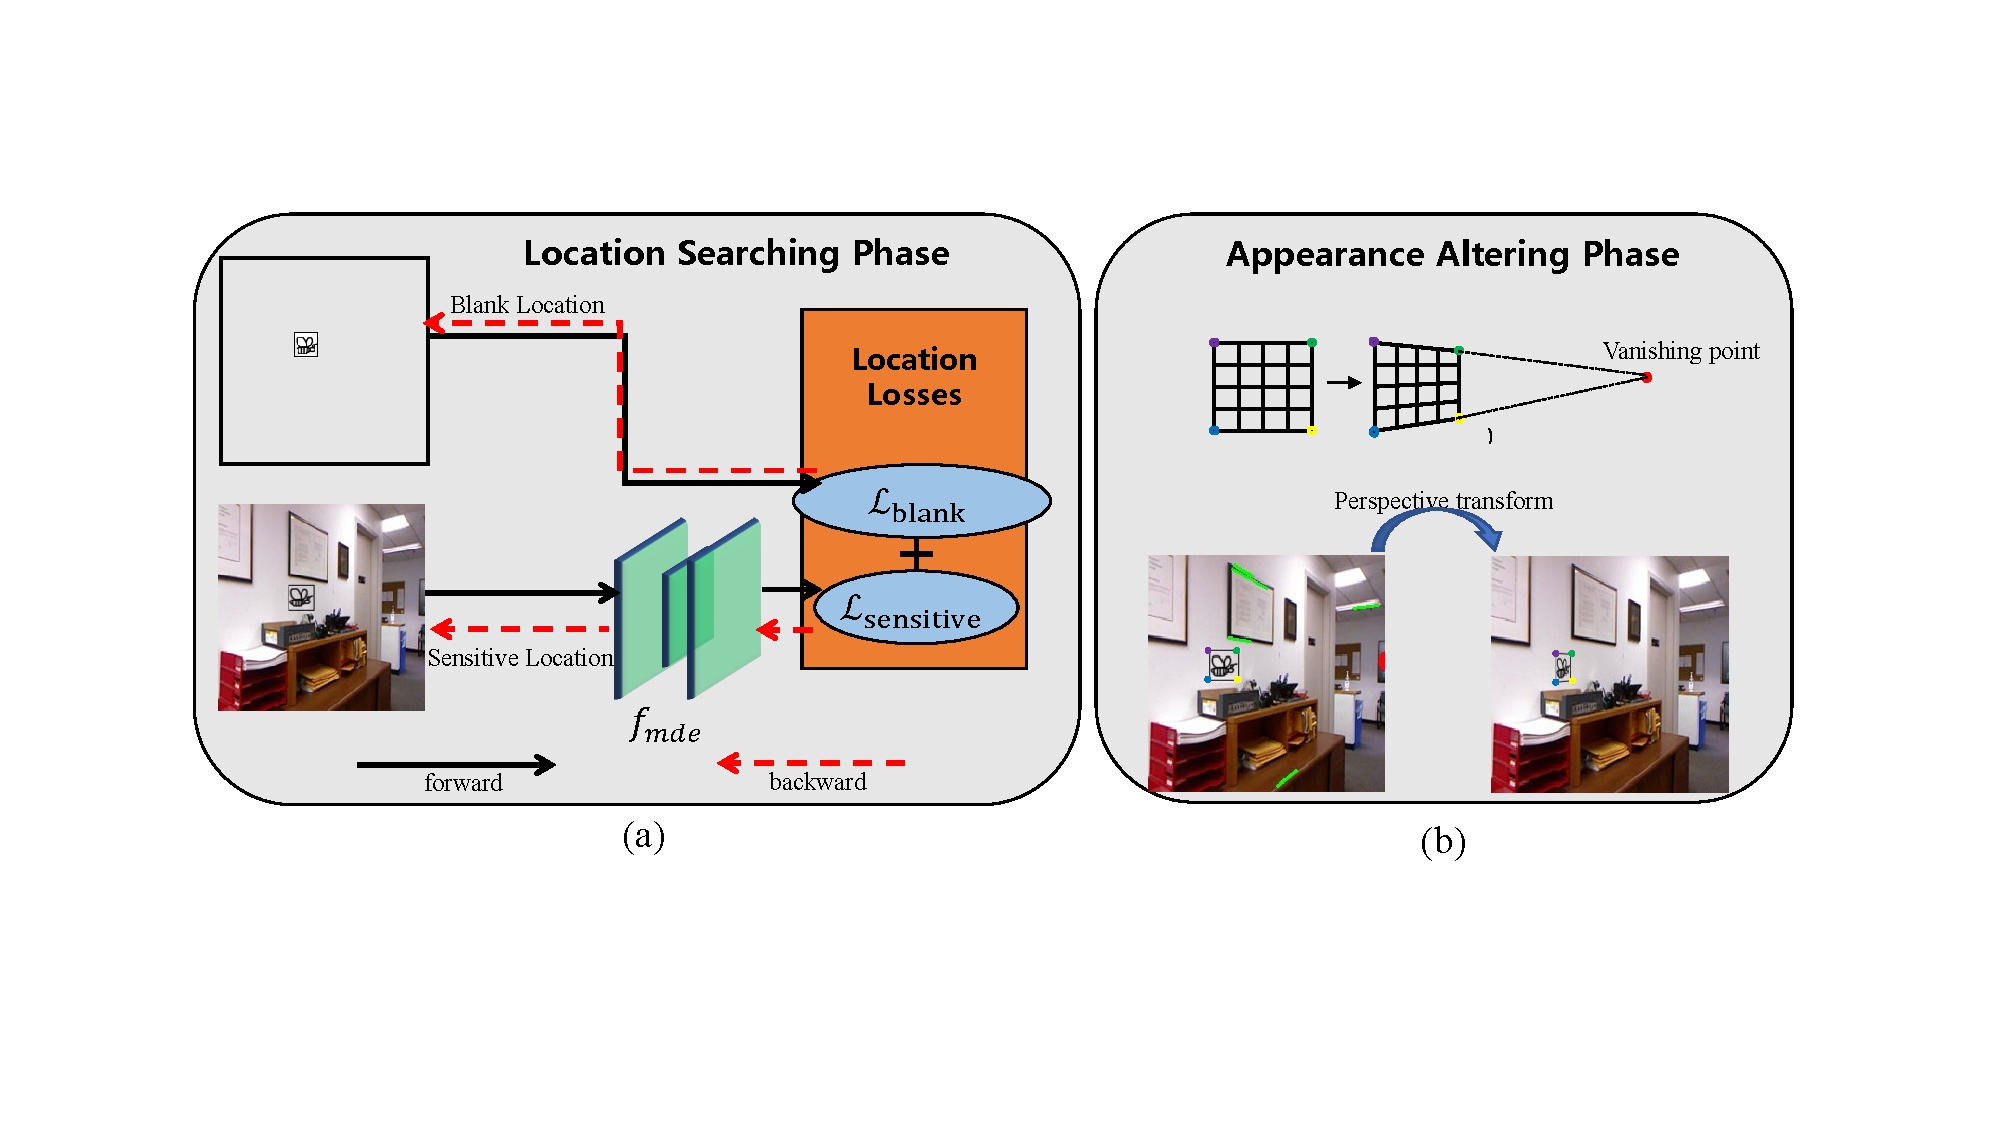
\includegraphics[width=1\textwidth]{imgs/stream.pdf}
	\caption{Stream of our MDE attacking method. 
	The whole stream consists of two phases: (a) location
	searching phase and (b) altering appearance phase.}
	\label[]{stream}
\end{figure*}
\subsubsection{Unsupervised}
Although there exist some datasets with ground truth depth 
annotation, dense and accurate depth maps are labor-consuming and rare. 
In that case, unsupervised methods dominate recently.
Godard et al.~\cite{Godard_2017_CVPR} exploit the left-right 
consistency of binocular image pairs
to tackle this issue: 
with a decently predicted disparity, 
the two images sampled from a binocular camera can synthesize each other. 
A consecutive vedio sequence can provide a constrain for MDE.
Given a middle frame and its former, later frame sampled from a video, 
DNNs can estimate the camera pose and the depth, with which we can 
restore the other two frames. Based on this constrain, camera pose 
and depth can be learned jointly~\cite{Zhou_2017_CVPR}.
However, there is a flaw in both video and binocular solutions.
On the one hand, binocular image pairs methods struggle in occlusion 
and texture-copy problems, yet, on the other hand, as an alternative method, 
predicting depth from a video performs unsatisfactorily 
when it comes to relatively stationary objects.
To address this, Godard et al.~\cite{Godard_2019_ICCV} proposed a multi-scale reconstruction
loss and a automasking approach to ignore relatively stationary objects.
\subsection{Patch Attack}
Adding perturbations to images has a limit: 
the imperceptive noise can not be captured by camera.
Recently, researchers turn to generating adversarial examples with
patches. It can be captured by camera and it can implement to physical
world. The only question is, how to make it concealed.

Sharif et al.~\cite{Sharif_2017_CCS} attacked FRS using real 
printed glass frames, 
with which the FRS can not recognize the person or recognize him
as someone else in the system. The pattern of these frames are 
generated by optimizing a composite objective function, 
including gradient decenting, smoothness of perturbations and 
non-printability score (NPS) optimal terms.
Tom et al.~\cite{Brown_2017_arxiv} abandon the camouflage of the attack, 
they attack DNNs with an apparent, universal patch, 
which is updated with different locations and transformations settings.
To generate robust adversaries, 
eykholt et al.~\cite{Eykholt_2018_CVPR} sampled from both 
actual physical and synthetic transformation images. Besides,
they found that there exist vulnerable and robust areas in an 
image and identified these areas by computing perturbations 
using the $L_1$ regularization. Then they generate perturbations 
using $L_2$ regularization on vulnerable areas, finally reshape 
the perturbations to a graffiti shape. In doing so, they achieve 
a high successful rate under various environmental conditions.
Liu et al.~\cite{Liu_2019_AAAI} also attacked the traffic signs. Instead of 
locating the vulnerable areas by computing, they locate 
the patch by a attention model, which takes as input the 
traffic sign, outputs an mask that indicates where to put the patch. 
The patch is generated through a GAN, which consists of a generator 
to generate a misclassification patch and a discriminator 
to discriminate whether the patch is original or adversarial. 
Kong et al.~\cite{Kong_2020_CVPR} also use a GAN to generate 
perturbation patches. 
In particular, they manipulate advertisement posters as original patch, 
which is artificially stuck on a street billboard after it 
through a GAN. This method produces better inconspicuousness yet 
the process of sticking the patch to billboard is labor consuming.
%The location of a patch matters to the camouflage. 
In~\cite{Hu_2021_ICCV}, the locations of patches are artificially 
determined and fixed
to make a better camouflage.
They first detect all humans in an image and pin a generated patch 
on their shirt. This attack makes the adversarial examples look as 
natural as a natural shirt pattern.
Forwardmentioned attack methods need to access to the objects they 
attacked. The advantage is that adversarial examples are more 
inconspicuous, it is hard to deployment in the physical world though. 
To this end, Zolfi et al.~\cite{Zolfi_2021_CVPR} proposed 
a contactless attack method. 
Several translucent patches are generated by updating the affine 
transformation matrix, then they are deployed on the camera's lens.

\section{Method}
In this section, we are going to present our 
MDE attacking method in detail. we first formulize the problem 
in Sec~\ref{Problem Statement}. 
Then we introduce how we design our patch to attack the MDE
system in Sec~\ref{Patch Design}. 
Finally we explain how the patches are optimized in 
Sec~\ref{Objective Function}.

\subsection{Problem Statement}
\label[]{Problem Statement}
Given a MDE data distribution:
$\mathbb{R}^{H\times W\times 3} \rightarrow \mathbb{R}^{H\times W}$, 
a MDE model $f_{mde}$ can learn a map that simulate the distribution 
within an error range. Considering elaborately designed 
perturbations can hardly be detected by consumer cameras, 
we are going to attack $f_{mde}$ by sticking inconspicuous 
patterns$\delta$ on appropriate areas. 
\begin{align}
	I^{'} = (1 - m) \odot I + \delta 
\end{align}
where$I$ is clean original image, $I^{'}$ is 
adversarial example, $m$ is a mask that covers
all non-zero pixels of the patch $\delta$. 
%Note that this is 
%a representation of attacking with one patch, 
%we adopt more than one patch in our 
%following experiments. 
Our goal, attacking a MDE system, is to 
maximize the error of ground truth depth map $D^{*}$ and 
depth map generated from $I^{'}$.
$\Vert \centerdot \Vert_p$ denotes the $l_p$ norm.
\begin{align}
	\max  \Vert f_{mde}(I^{'}) - D^{*} \Vert_{p}
\end{align} 
%Different with former works, we do not use patches generated by 
%adding perturbations or through a GAN, we simply use a 
%perspective transformation matrix $T$ to update the location and 
%shape of the patch to make it 
%more destructive, more concealed, meanwhile, save 
%more optimization time.
%Our final definition of the adversarial examples is:
%\begin{align}
%	I^{'} = (1 - m) \odot I + T\delta 
%\end{align}

\subsection{Patch Design}
\label[]{Patch Design}

\paragraph{location}
%Current works leverage a GAN to add perturbations on patterns or 
%generate patterns, which has more time and spatial complexity. 
%In this section, we will introduce our fast and light optimal 
%method in detail, which searches the most destructive area and 
%transforms the patches to a more rational style before sticking.
To obtain an adversarial example $I^{adv}$,
the first problem we encountered is where to stick the patches.
Exhaustive search is feasible but time consuming. We expect to
complete this this process automatically and quickly.
So we turn to optimizing the patch location 
by gradient decenting.  
We define a $2 \times 3$ matrix 
$\mathbf{A}_\theta$ for each patch to implement this 
location search process.
By optimizing this $\mathbf{A}_\theta$, a patch can update its 
location automatically.
\begin{align}
	\left[
		\begin{array}{ccc}
			1 & 0 & t_x \\
			0 & 1 & t_y \\
		\end{array}
		\right]      
\end{align}
where $[t_x,t_y]^\top$ denote the offsets $O$ in 
horizontal and vertical directions, respectively. 
Initial values are $[0,0]$, which represent
that the center of the patch is on the center of the image.


Specifically, we first place the patch $\delta$
in the center of the 
clean image $I$,
then pad 0 around it to the size of $I$.
The homogeneous coordinate of this 
patch is noted as $G$ and its size is $H\times W\times 3$.
For each pixel of padded $\delta$, $G_i = (x_i, y_i, 1)$.
This location searching process can be represented as:
\begin{align}
	{G'}^T = A_{\theta}~{G}^T
\end{align}
\begin{align}
	\label[]{new coordinate}
\begin{pmatrix}
	x_s\\
	y_s	
	\end{pmatrix} = 
		\left[
			\begin{array}{ccc}
				1 & 0 & t_x \\
				0 & 1 & t_y \\
			\end{array}
			\right] 
			\begin{pmatrix}
				x_t\\
				y_t\\
				1	
				\end{pmatrix} 
\end{align}


%$[m,n] \in [-1,1]$ denote the perspective parameters.
%Given a monocular image $I \in \mathbb{R}^{H\times W\times 3}$,
%the pixel coordinates form a grid$H \times W \times 2$.

\paragraph{Appearance}
The location problem is settled by optimizing an
affine transform matrix
$\mathbf{A}_\theta$,
next we address altering the appearance of the patch.
The appearance altering phase can be seen in 
Fig~\ref{stream}(b).

When we alter the appearance of the patch, 
for better visualization quality, we followed 
the principle of perspective drawing: 
the vanishing point is where all parallel lines 
intersect and is always on the horizon line.
Fig~\ref{perspective} clearly 
illustrates this principle.
\begin{figure}
	\centering
	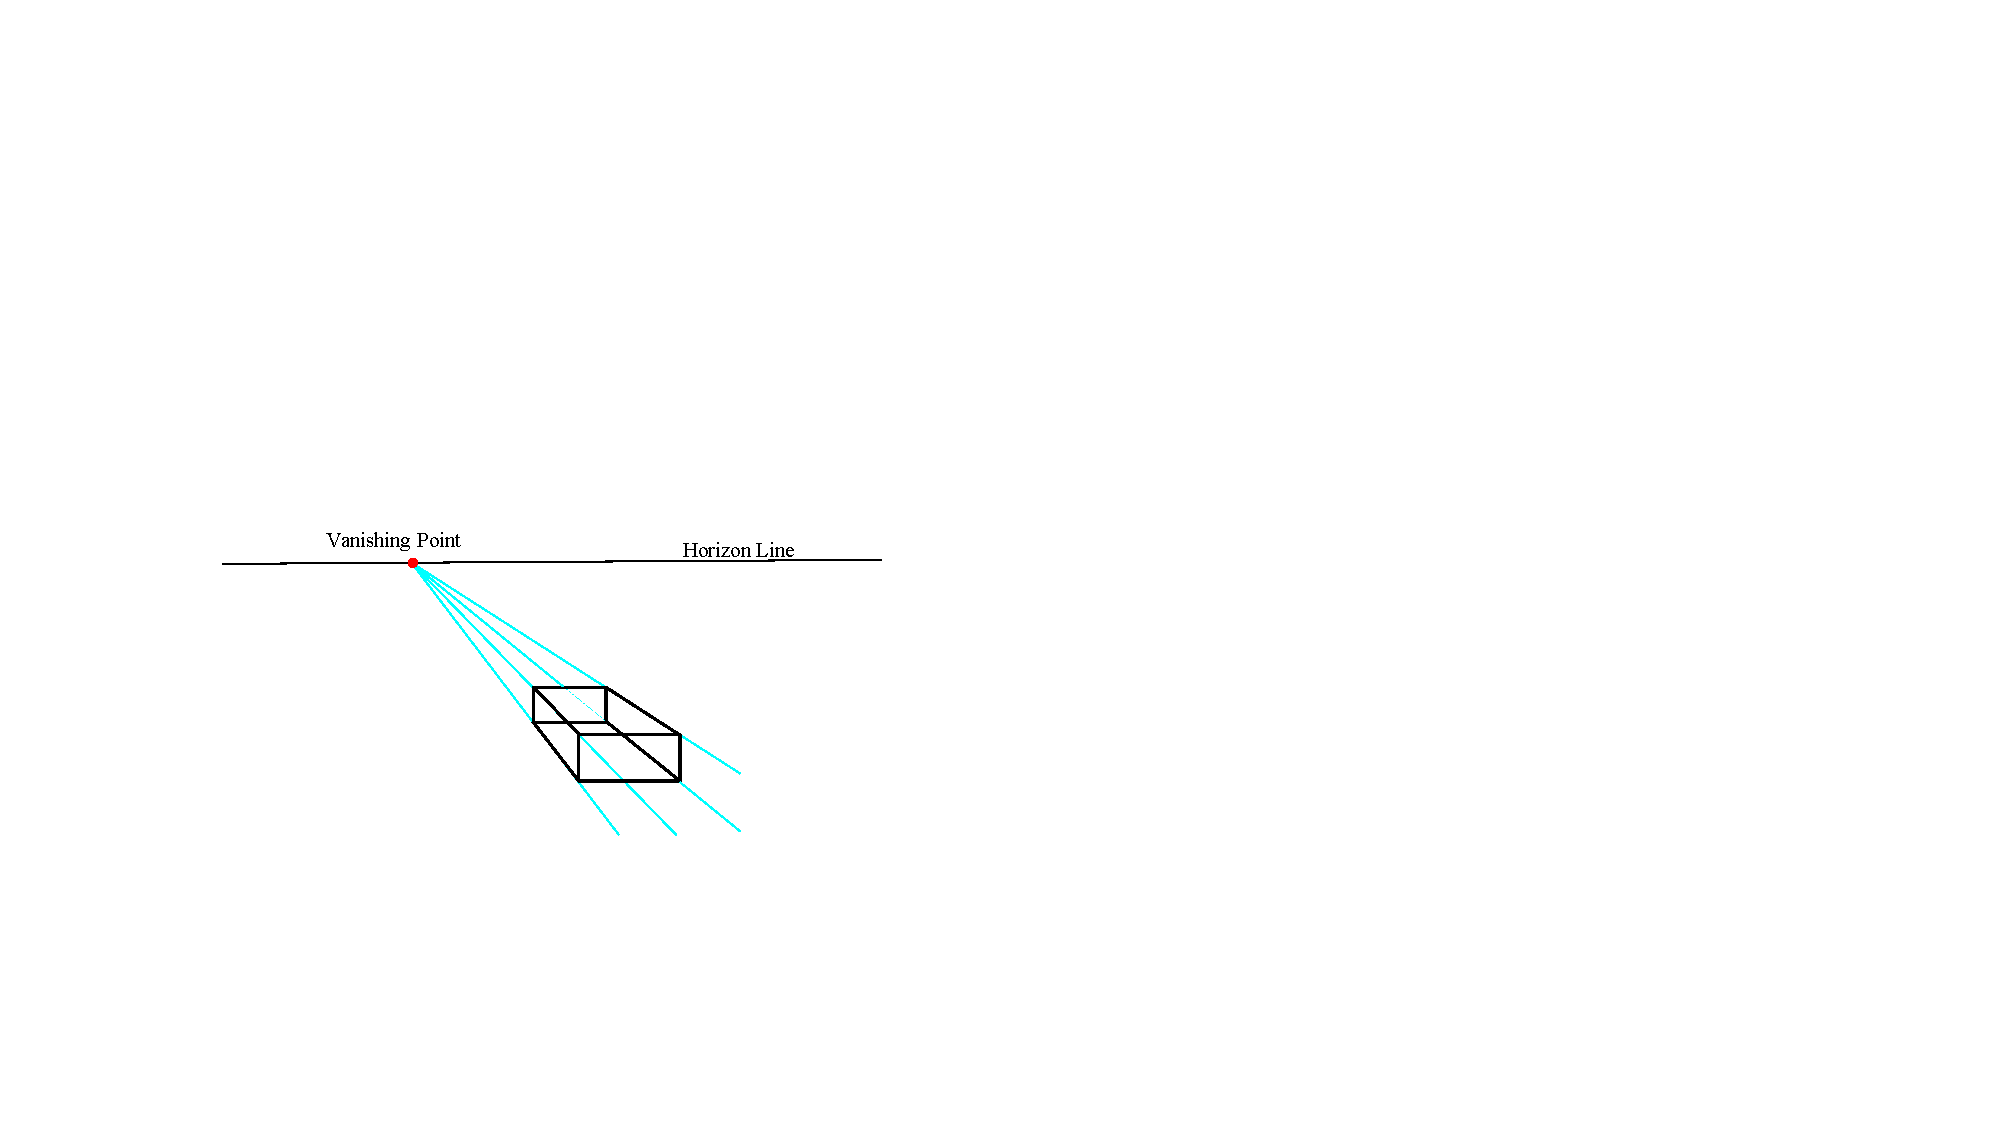
\includegraphics[width=1\linewidth]{imgs/perspective.pdf}	
	\caption{Diagram of single point perspective drawing:
	All the vanishing lines lead to the vanishing point.
	The horizontal and vertical lines, however, 
	remain parallel to each other.}
	\label[]{perspective}
\end{figure}

We first detect straight lines in the attacked 
scene with \textit{Hough} transform, then we obtain 
the vanishing point by extending this lines 
and computing their intersection.
Based on the principle of perspective drawing, as illustrated
in Fig~\ref{stream}(b), if we connect the left-top point and 
vanishing point, the right-top point should lay on this 
line. Same on the bottom line.
Meanwhile, the connection lines, which converge to vanishing
points, will look shorter than their original length. 
We explain this fact in Fig~\ref{stream}(b):
when seen from the front
view, the width of patches $w$ will shrink to $w'$.
\begin{align}
	w' = \sqrt{w^2-d^2}
\end{align}
Since this task we concentrate on is just MDE, we possess
the depth of each pixel. 
The patches' depth $d$ can be
got by subtracting fronter boarder depth from 
back boarder depth. We set $w=0.1m$ in our experiments.
We get four corrected corner coordinates, with which we 
alter the appearance of the patch. The perspective
transforms in this phase are implemented with 
\textit{OpenCV}. 

\subsection{Objective Function}
\label[]{Objective Function}
The aim of this research is to attack MDE models inconspicuously 
with patches, we consider three factors: attack effect, 
which area of the adversarial example is more inconspicuous 
and what appearance of the patches are more 
inconspicuous.
The last consideration about the appearance is addressed
by perspective geometry, while the attack effect and 
inconspicuous areas are optimized by two loss funtions
respectively.
The two loss functions consisit 
our objective function in a linear manner:
\begin{equation}
\begin{aligned}
	&\mathcal{L}_{total} = \lambda_1\mathcal{L}_{attack} +
	\lambda_2\mathcal{L}_{blank}\\ 
\end{aligned}
\end{equation}
We are going to explain the two loss functions in the following
part of this section.

\subsubsection{attack effect}
MDE $f_{mde}$ systems generate depth maps, whose pixel values 
represent the distance from area to sample sensors.
To obtain best attack effect, that is, 
to maximize the error between prediction maps and annotated maps:
\begin{align}
\mathcal{L}_{attack} = \Vert f_{mde}(I^{'}) - D^{*} \Vert_{p}
\end{align}
We use $L_1, L_2$ and Huber loss in our experiments.

\subsubsection{Visualization Quality}
For better inconspicuousness, we camouflage the patch 
as graffiti, which can be usually found on 
blank walls. Blank means with no pictures, marks or 
decoration on white walls.
Based on this we design Blank loss to help the patch to 
find blank areas, the Blank loss
consisits of two optimization sub-terms:
	\begin{align}
		\label[]{blank}
		\mathcal{L}_{blank} = \mathcal{L}_{smooth}+\mathcal{L}_{white}
 	\end{align}
$\mathcal{L}_{smooth}$ constrain the patch locate
on areas with low texture complexity:
	\begin{align}
		\label[]{smooth}
		\mathcal{L}_{smooth} = 
		-\frac{\sqrt{\partial_x (M \odot I) + \partial_y (M \odot I)}}{N} 
 	\end{align}
where $M$ denotes a full 1 mask that has the 
same size as $\delta$. $\partial_x$ and $\partial_y$
denote the gradient in $x$ and $y$ directions respectively.
$N$ is the number of pixels in $M$.
$\mathcal{L}_{white}$ constrain the patch locate
 on white areas:
	\begin{align}
		\label[]{white}
		\mathcal{L}_{white} = \frac{\sum_{1}^{N} M \odot I}{N} 
 	\end{align}

\subsection{location Optimization}
As indicated in Eq.\ref{new coordinate},
the coordinates of the target pixels $G'_i$ are continuous values. 
We adopt bilinear interpolation to determine the value of 
the target pixel. 
Bilinear interpolation mechanism is proved 
to be differentiable in 
\textit{spatial transformer networks}~\cite{stn}.
By maximizing the $\mathcal{L}_{attack}$, 
we can optimize the offsets $O$ step by step.
\begin{align}
	O_{S+1} = Clip 
	\{O_{S} + \alpha 
	{\bigtriangledown_{O}\mathcal{L}_{total}}\}. 
\end{align}
The stream of location searching phase can be seen in 
Fig~\ref{stream}(a). 

\section{Experiments}
\begin{figure*}[htb]
	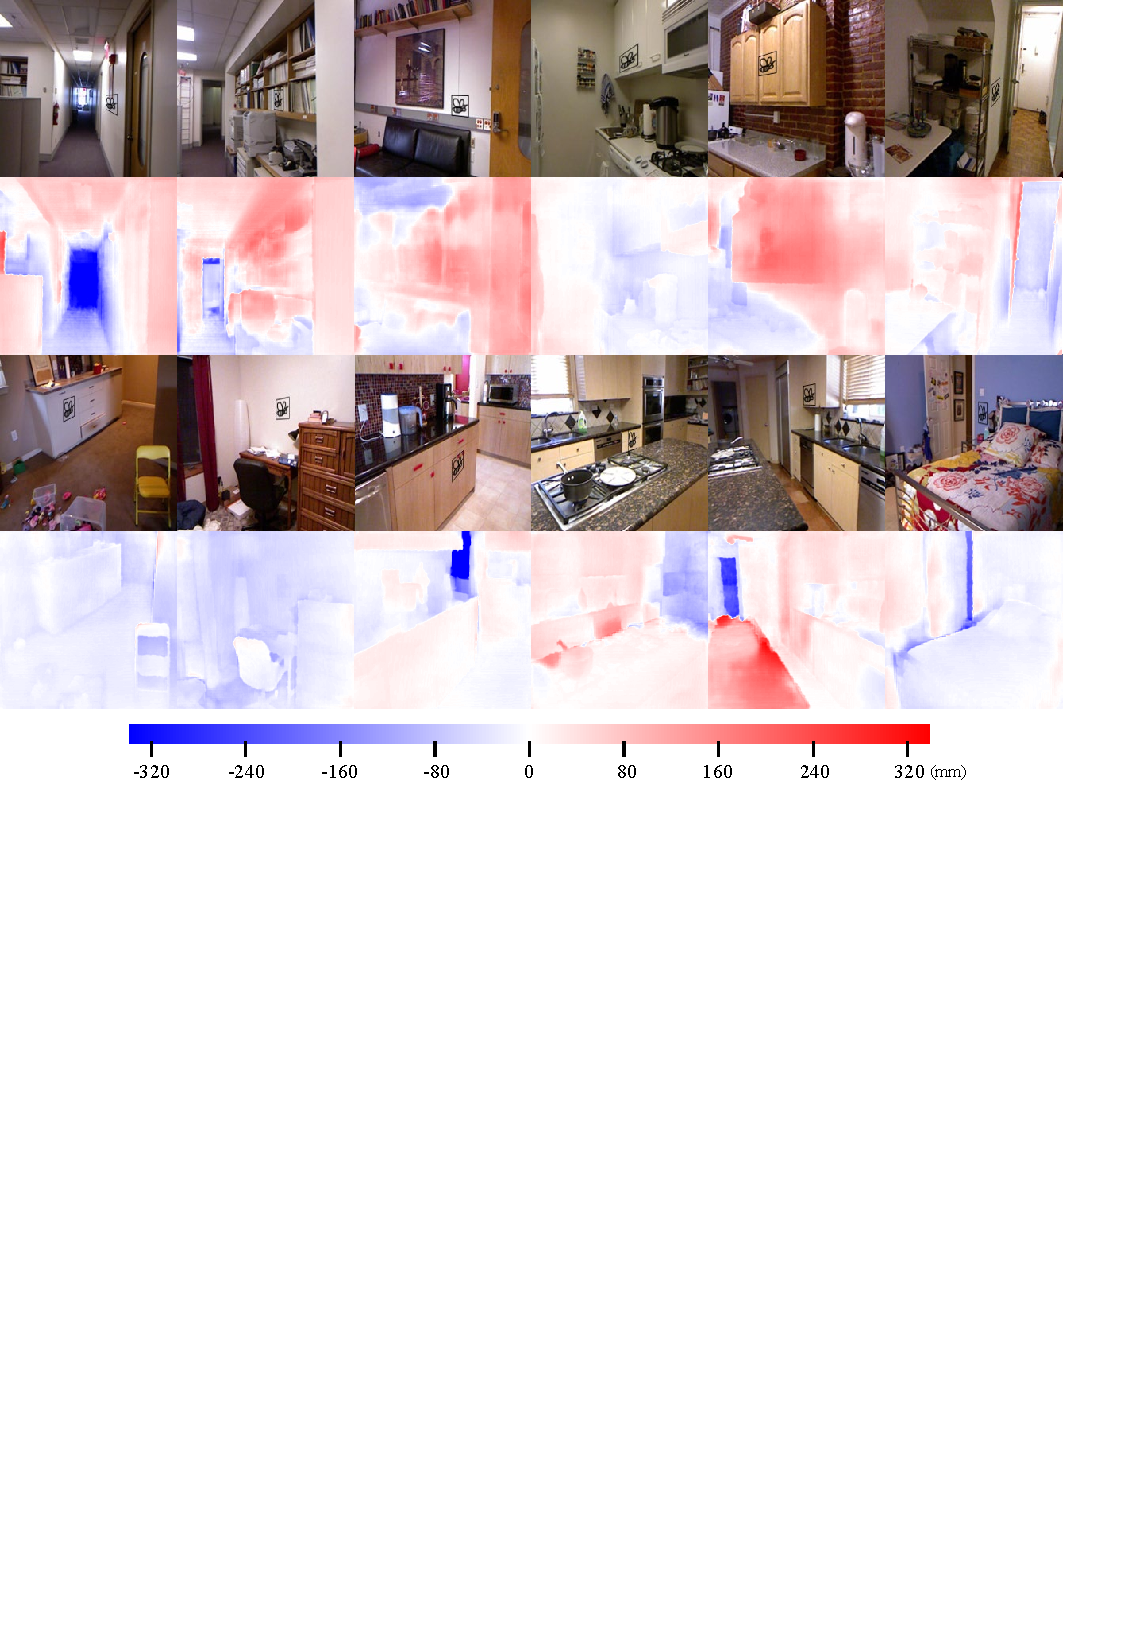
\includegraphics[width=1\textwidth]{imgs/results.pdf}
	\caption{The visualization of our patch attack
	method. The first and third rows are $I^{adv}$.
	The second and fourth rows are the visualization
	of prediction error: 
	$f_{mde}(I^{adv}) - D^{*}$.
	The color bar down the results explicates the 
	error value intuitively.
	We emphasize the patches using surrounding 
	black boxes, which are transformed in the 
	altering appearance phase also.}
	\label{results}
\end{figure*}
In this section, we conduct several experiments to exhibit 
the results of our automatic and inconspicuous attack
method on the fastdepth~\cite{Wofk_2019_ICRA} MDE system. 
%As mentioned before, we consider three factors: attack effect, 
%which area of the adversarial example is more inconspicuous 
%and how to make the patches more 
%inconspicuous. 
We introduce our implemention detail, including datasets,
data pre-processing and experiment environment in
Sec~\ref{Implemention Detail}.
In Sec~\ref{Visualization Attack Results} and 
Sec~\ref{Quantitative Attack Results}, 
our attack effects are shown by visualization
and quantitative comparison.
Then we demonstrate the automatic searching process driven 
by our method in Sec~\ref{Automatic Searching}. Finally we
show and analyze the visual quality of our adversarial examples. 

\subsection{Implemention Detail}
\label[]{Implemention Detail}
For the MDE system, we use Fastdepth~\cite{Wofk_2019_ICRA}. 
We also use the same dataset NYU Depth v2
~\cite{Silberman_2012_ECCV} used in
the Fastdepth~\cite{Wofk_2019_ICRA}. 
This dataset is an indoor dataset, whose depth range is 
0-10 m.
It consisits of 1449 densely annotated depth and RGB images pairs,
795 of which are split to train dataset and the rest are
split to test dataset.
For the image pre-processing, we followed the process in
Fastdepth: images are resize to $250 \times 333$ firstly, 
secondly, center cropped to $224 \times 304$, in the end 
they are resized to $224 \times 224$.

For the patch dataset, we choose QuickDraw~\cite{quickdraw}.
QuickDraw is a collection of 50 
million hand-writing drawings across 345 categories.
We select several categories, including bee, ant,
dolphin, crocodile and so on. The size of them are
all $28 \times 28$.

In our experiments we set 
$\alpha = 0.002$, total optimization step is 300 steps.
To avoid overflow from RGB images, $O$ are
clipped between $(-0.875,0.875)$.
Our experiments are performed on an 
NVIDIA GeForce RTX 2080 TI GPU.
%®
\subsection{Visualization Attack Results} 
\label[]{Visualization Attack Results}
As mentioned above, our method generate 
inconspicuous and destructive $I^{adv}$.
The results are shown in Fig~\ref{results}
from the two aspects. 

For inconspicuousness, we show the adversarial examples
in the first and third rows. The black box shows that
our adversarial examples follow the principle 
of perspective drawing. Besides the patches lay on 
walls and furniture, which makes our examples look like 
graffiti and more harmonious in indoor scenes.

For destructiveness, we show the 
prediction error in the sencond and fourth row.
Our method achieves $320mm$ max error. Prediction results
from $I^{adv}$ are usually nearer than ground truth 
depth maps in far-range areas, for instance, 
the blue areas in Fig~\ref{results}.
However, the results are farther in near-range areas,
which means our adversarial examples mislead the MDE 
system and make the prediction results converge to 
middle distances.

\subsection{Quantitative Attack Results} 
\label[]{Quantitative Attack Results}
\begin{table*}
    \centering  % 显示位置为中间
    \caption{Accuracy of different attack method and original method}  % 表格标题
    \label{table1}  % 用于索引表格的标签
    %字母的个数对应列数,|代表分割线
    % l代表左对齐,c代表居中,r代表右对齐
    \begin{tabular}{c|c|c|c|c|c|c}  
		\toprule
      \multicolumn{2}{c|}{}&RMSE&MAE&absrel&delta1&Runtime \\  % 表格中的内容,用&分开,\\表示下一行
      \midrule
      %& & & \\[-6pt]  %可以避免文字偏上 
      \multicolumn{2}{c|}{fastdepth}&0.600&0.427&0.162&0.771& \\
      \hline  % 表格的横线
      \multirow{3}{*}{Ours}&l1&0.608&0.431&0.165&0.769& \\
      					&l2&0.608&0.431&0.165&0.769& \\
      					&Huber&0.608&0.431&0.165&0.769& \\
		\bottomrule
    \end{tabular}
  \end{table*}

\subsection{Automatic Searching} 
\label[]{Automatic Searching}
In this section you are going to find that given an image 
our attack method can search the sensitive zone and stick
the patch on the zone. To better demonstrate our search effect, 
we calculate the MAE 
maps of test images. Beginning from the left top corner, 
where is (-0.875,-0.875), we use strides 7 to move the patch 
step by step and calculate 
the MAE of each position, finally getting the MAE maps.
The red and violet colors in the maps represent higher and lower 
MAE values, respectively.
As you can see from Fig~\ref{patch_on_scenes}, 
our method can accurately search the sensitive area of the image.
Note that to emphasize our search effect, we didn't use the 
Blank (eq~\ref{blank})
loss function in this experiment. 
\begin{figure*}
	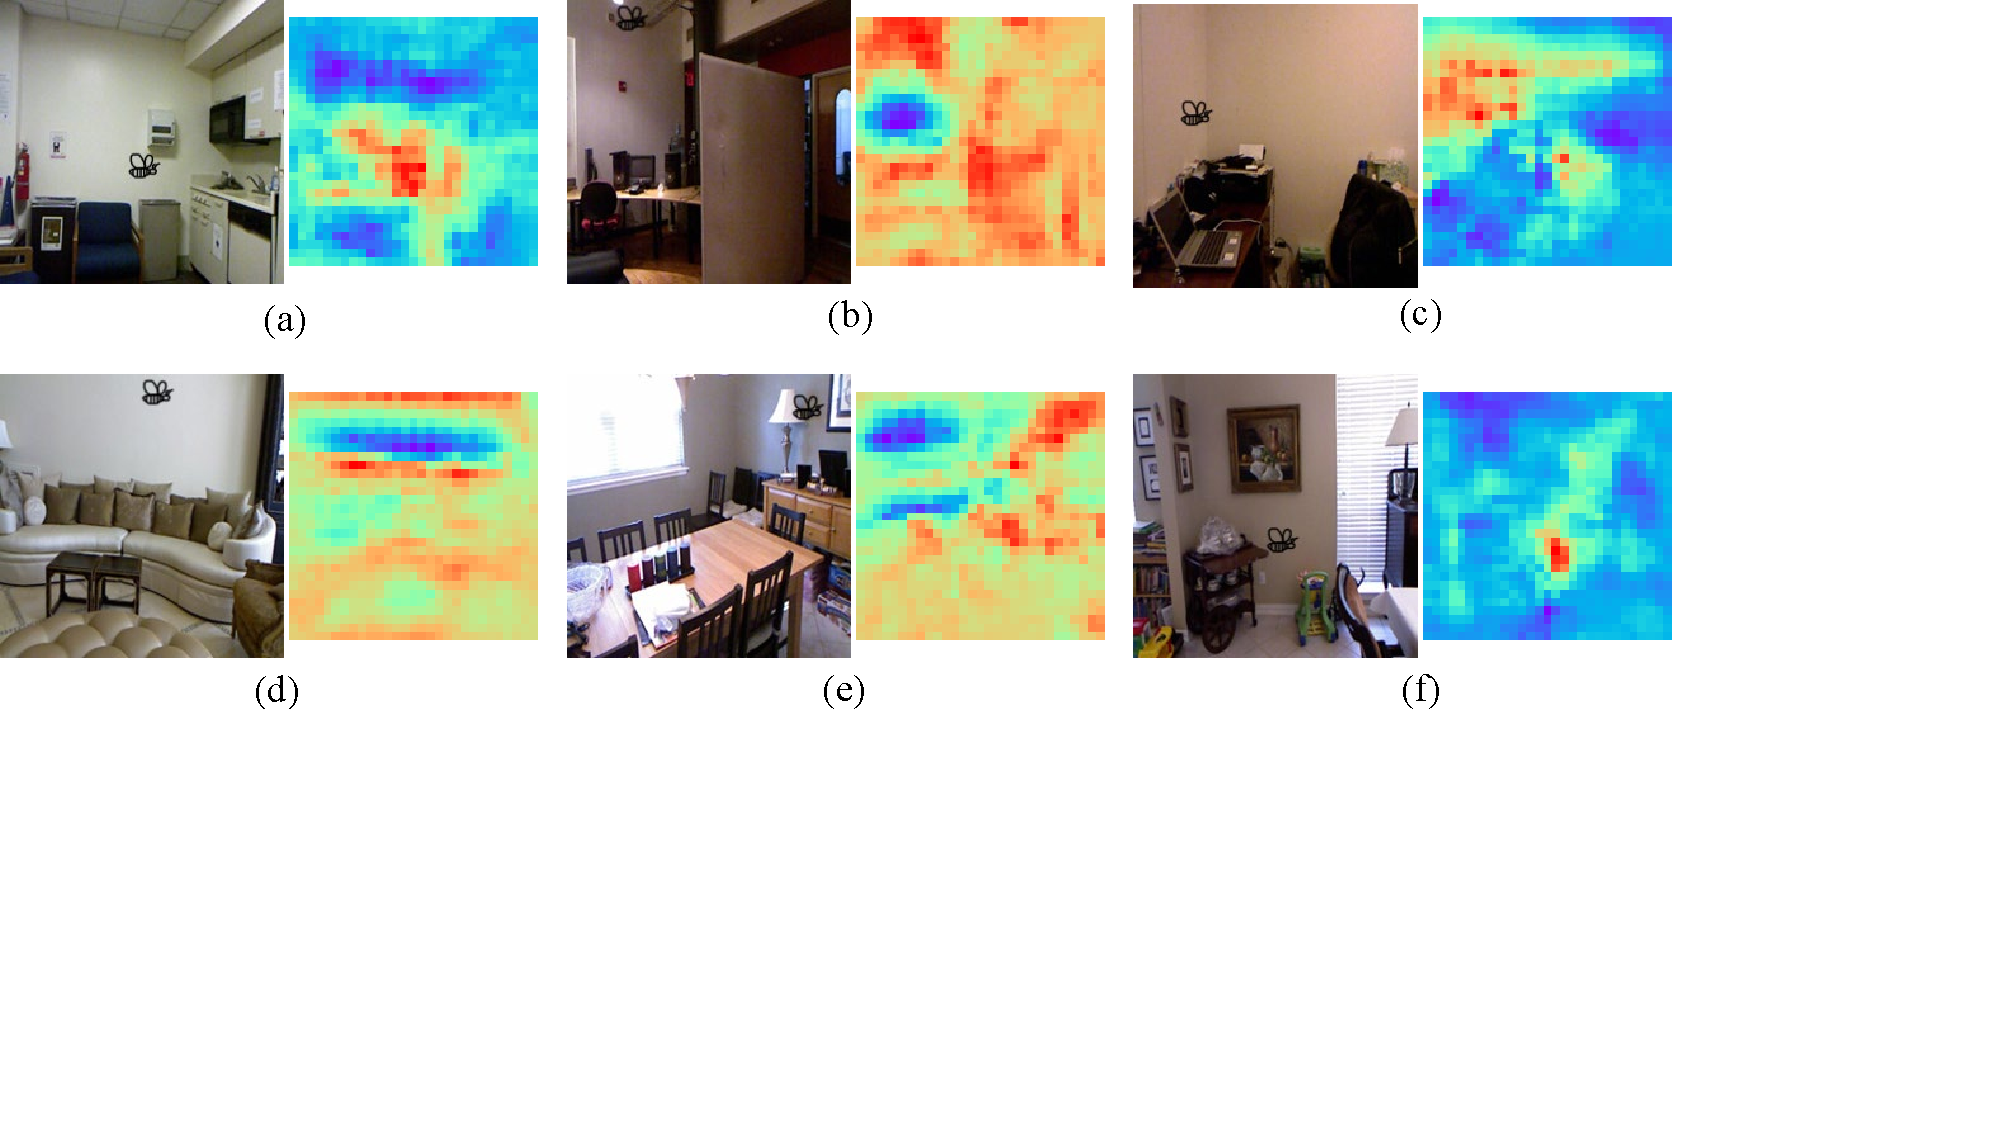
\includegraphics[width=1\textwidth]{imgs/patch_on_scenes.pdf}
	\caption{The final attack locations searched by our method (left) 
	and corresponding MAE maps (right). 
	The offsets of the maps are clamped between -0.875 and 0.875, 
	as a contrast,
	the width and height of the RGB images extend from -1 to 1,
	which makes the maps a little smaller than the RGB images.
	}
	\label[]{patch_on_scenes}
\end{figure*}

We visualize the serach path in Fig~\ref{search_path}.
\begin{figure*}
	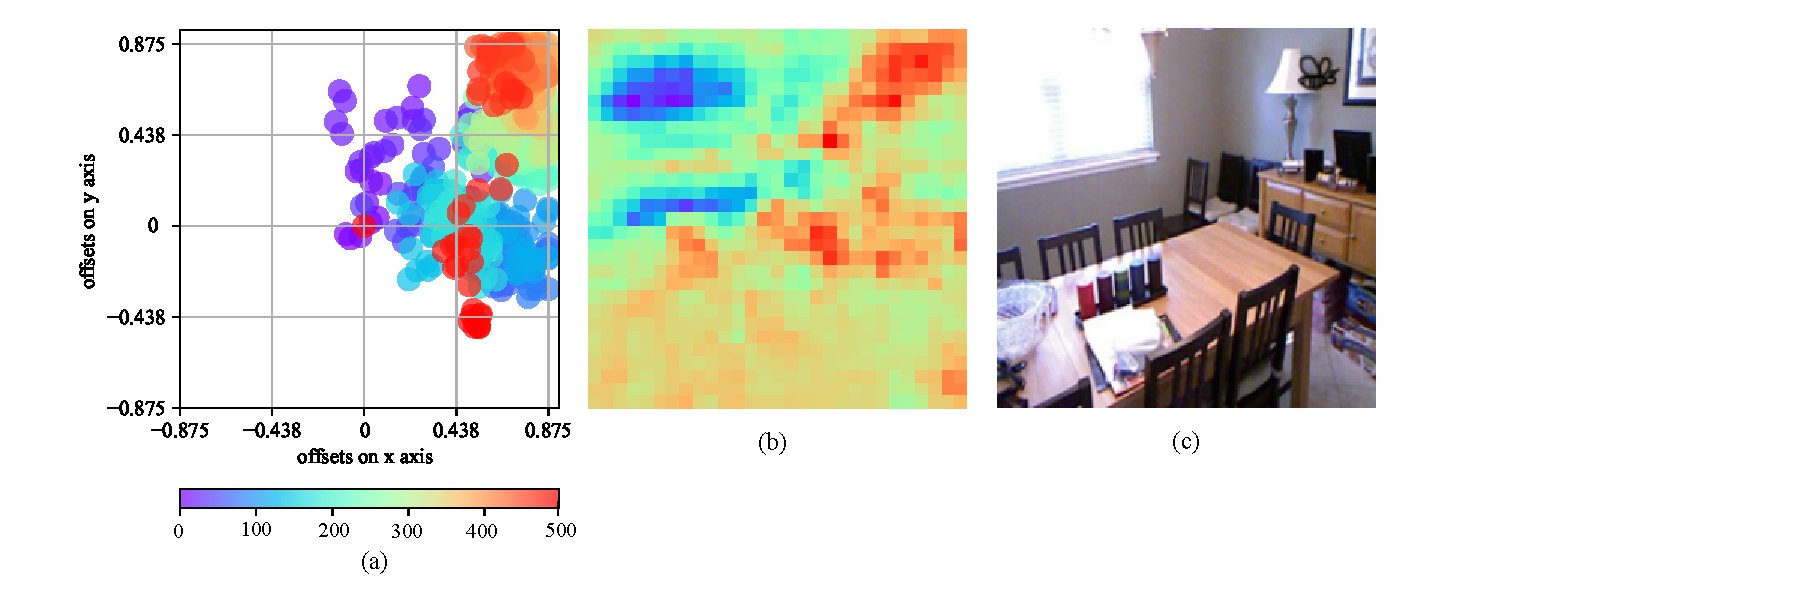
\includegraphics[width=1\linewidth]{imgs/search_path.pdf}
	\caption{The search path of~\ref{patch_on_scenes} (e), the
	color from violet to red represent the search steps from 0
	to 500.}
	\label[]{search_path}
\end{figure*}

We use different stickers to calculate their MAE maps on the 
same image, to investigate the impact of different patches on 
the sensitive area's location in the image. As shown 
in Fig~\ref{patches_on_one_scene}, the distribution of sensitive 
and robust areas in (c)~(f) is similar, the sensitive areas
are concentrated in the center, among them
(d) and (f) almost looked the same. However there are 
some differences between (h),(g) and (c)~(f). Intuitively, 
this is caused by the variations of patch\ding{176} and 
\ding{177} in saptial structure. Based on this, 
we conclude that, to similar patches, the distribution 
of an image's sensitive and robust area is usually the same. 
The similarity is more significant along with the smaller size. 

\begin{figure*}
	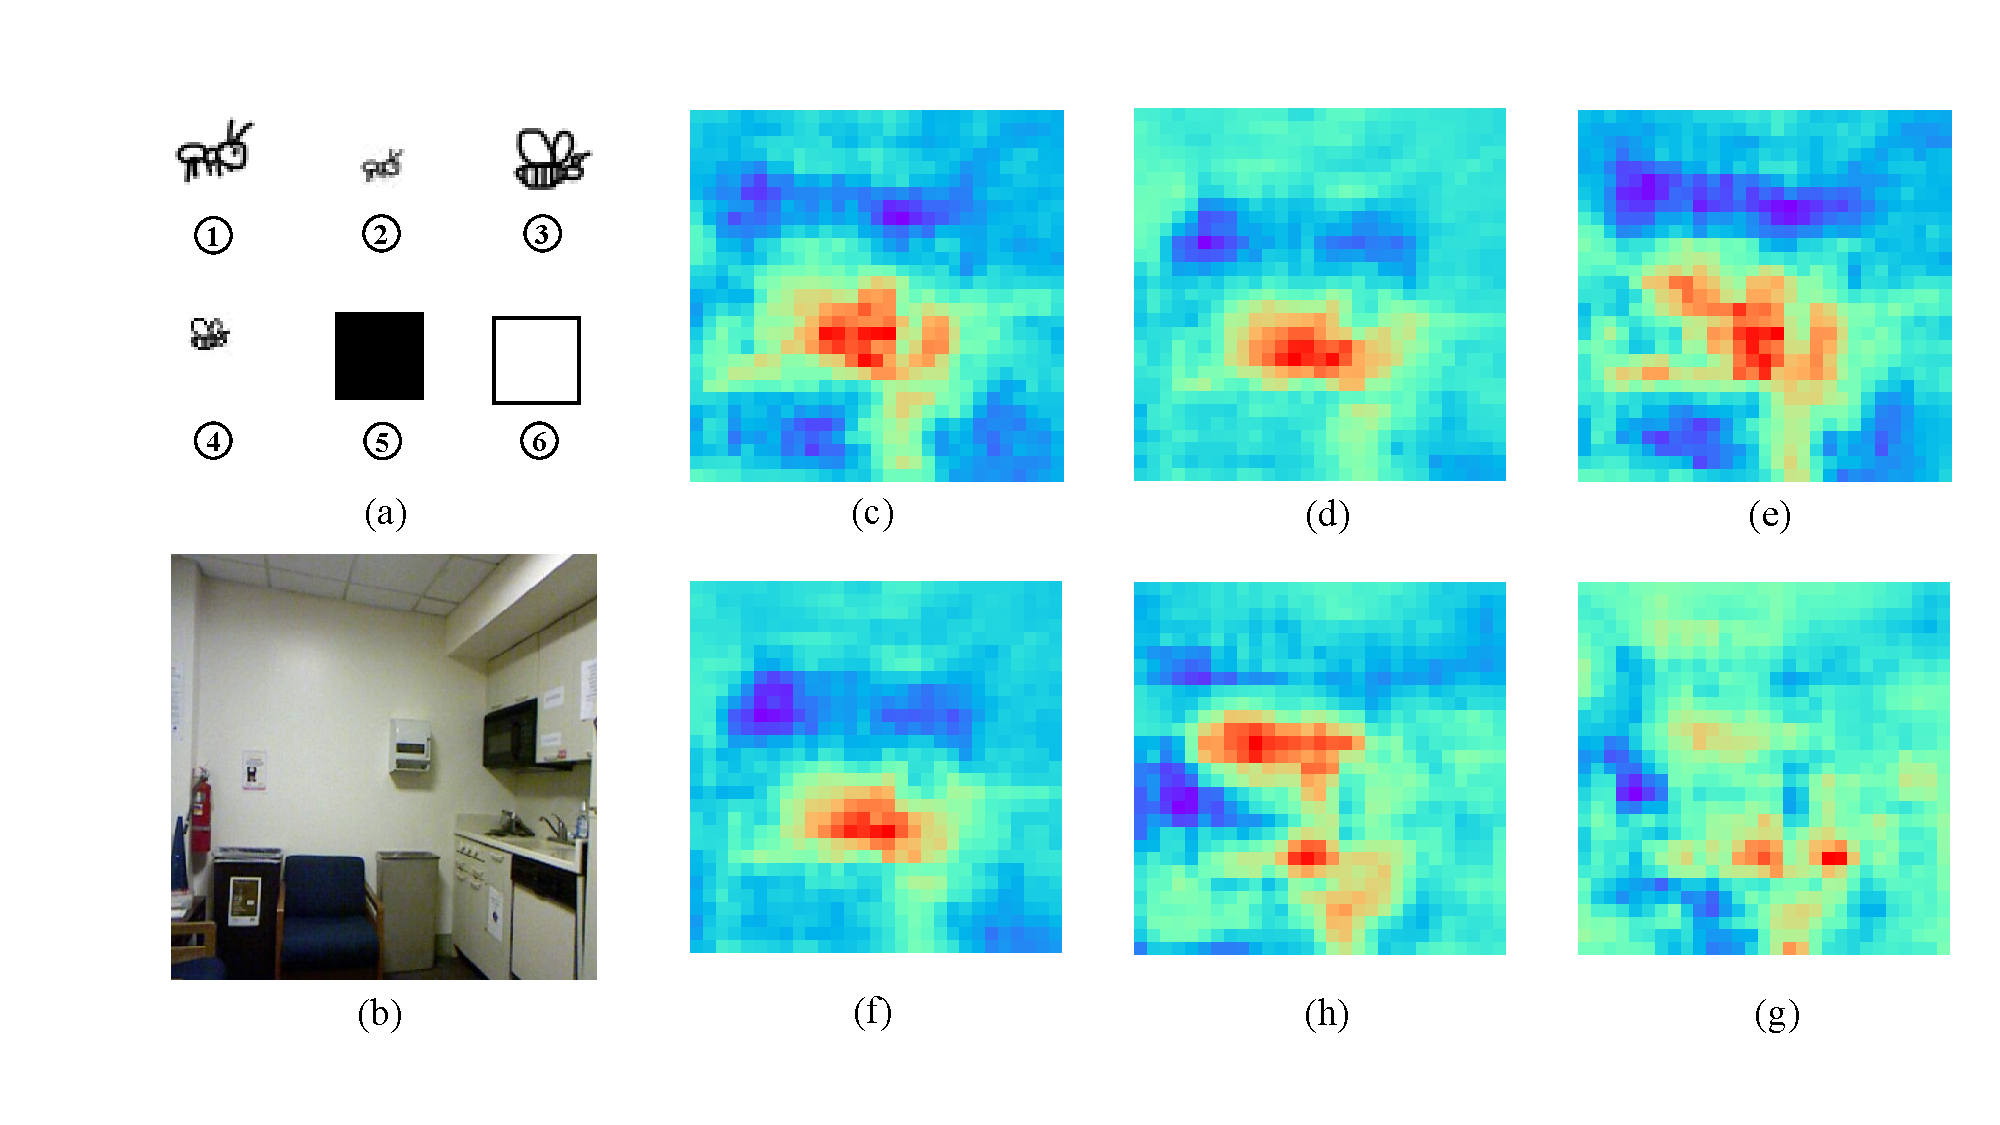
\includegraphics[width=1\linewidth]{imgs/patches_on_one_scene.pdf}
	\caption{There are 6 different
	patches in (a), they are stuck in (b) to 
	calculate MAE maps (c~g). The placement of (c~g) is the same 
	as the patches' placement in (a). Patch \ding{173} and \ding{175}
	are down sampled from \ding{172} and \ding{174} with factor 0.5.
	Patch \ding{176} is a black patch filled with 0 and patch 
	\ding{177} is a white patch filled with 1.
	The black box is for visualization this white patch.}
		
	\label[]{patches_on_one_scene}
\end{figure*}

\subsection{Visual Quality} 
\label[]{Visual Quantity}

\section{Conclusion}

%%%%%%%%% REFERENCES
{\small
\bibliographystyle{ieee_fullname}
\bibliography{egbib}
}

\end{document}
